\chapter{Das Prinzip von Gasdetektoren}

\noindent Gasgefüllte Detektoren sind eine effiziente Methode zur Untersuchung ionisierender Strahlung und physikalischer Wechselwirkungen, die zu Teilchenzerfällen führen. Das Verständnis ihrer Funktionsweise und ihrer inhärenten Grenzen erfordert die Diskussion der ihnen zugrundeliegenden physikalischen Mechanismen. In diesem Kapitel wird daher die Funktionsweise von Gasdetektoren auf Basis dieser Prinzipien erläutert.

	\section{Wechselwirkungen von ionisierender Strahlung mit Materie}
	Ionisierende Strahlung kann mit dem durchstrahlten Medium wechselwirken und so Ionisationen verursachen. Die Wechselwirkungen unterscheiden sich für Photonen und geladenen Teilchen, masselose, neutrale Teilchen haben demnach andere Wechselwirkungsmechanismen als geladene Teilchen: Geladene Teilchen deponieren den Großteil ihrer Energie durch inelastische Stöße mit den Elektronen des Materials \cite{Leo}. Dieser Prozess hinterlässt eine Spur von Elektron-Ion-Paaren im Material, was prinzipiell eine Rekonstruktion der Teilchenspur ermöglicht, und so beispielsweise die Analyse von Zerfallsprozessen erlaubt.\\
	\\
	Da die Spurrekonstruktion in dieser Arbeit keine zentrale Rolle spielt, werden im Folgenden die relevanten Wechselwirkungsphänomene fokussiert behandelt. Eine umfassende und detaillierte Behandlung der Teilchenwechselwirkungen findet sich exemplarisch in \cite{Leo} und \cite{Sauli_Multiwire}.

	\subsection{Photonen in Materie} \label{chap:Photonen}
	Die Wechselwirkung von Photonen mit Materie belaufen sich im Wesentlichen auf den photoelektrische Effekt, Compton-Streuung und Paarbildung. Die Wahrscheinlichkeit dieser Prozesse hängt vom Material und der Photonenenergie $E_{\gamma}$ ab. Abbildung \ref{fig:WirkungsquerschnittePhotonen} veranschaulicht diesen Zusammenhang, indem sie die Übergangsbereiche darstellt, in denen die einzelnen Prozesse in Abhängigkeit von der Kernladungszahl und der Photonenenergie dominieren. Im Folgenden werden diese Prozesse kurz erläutert:
	\begin{figure}[h]
		\centering
		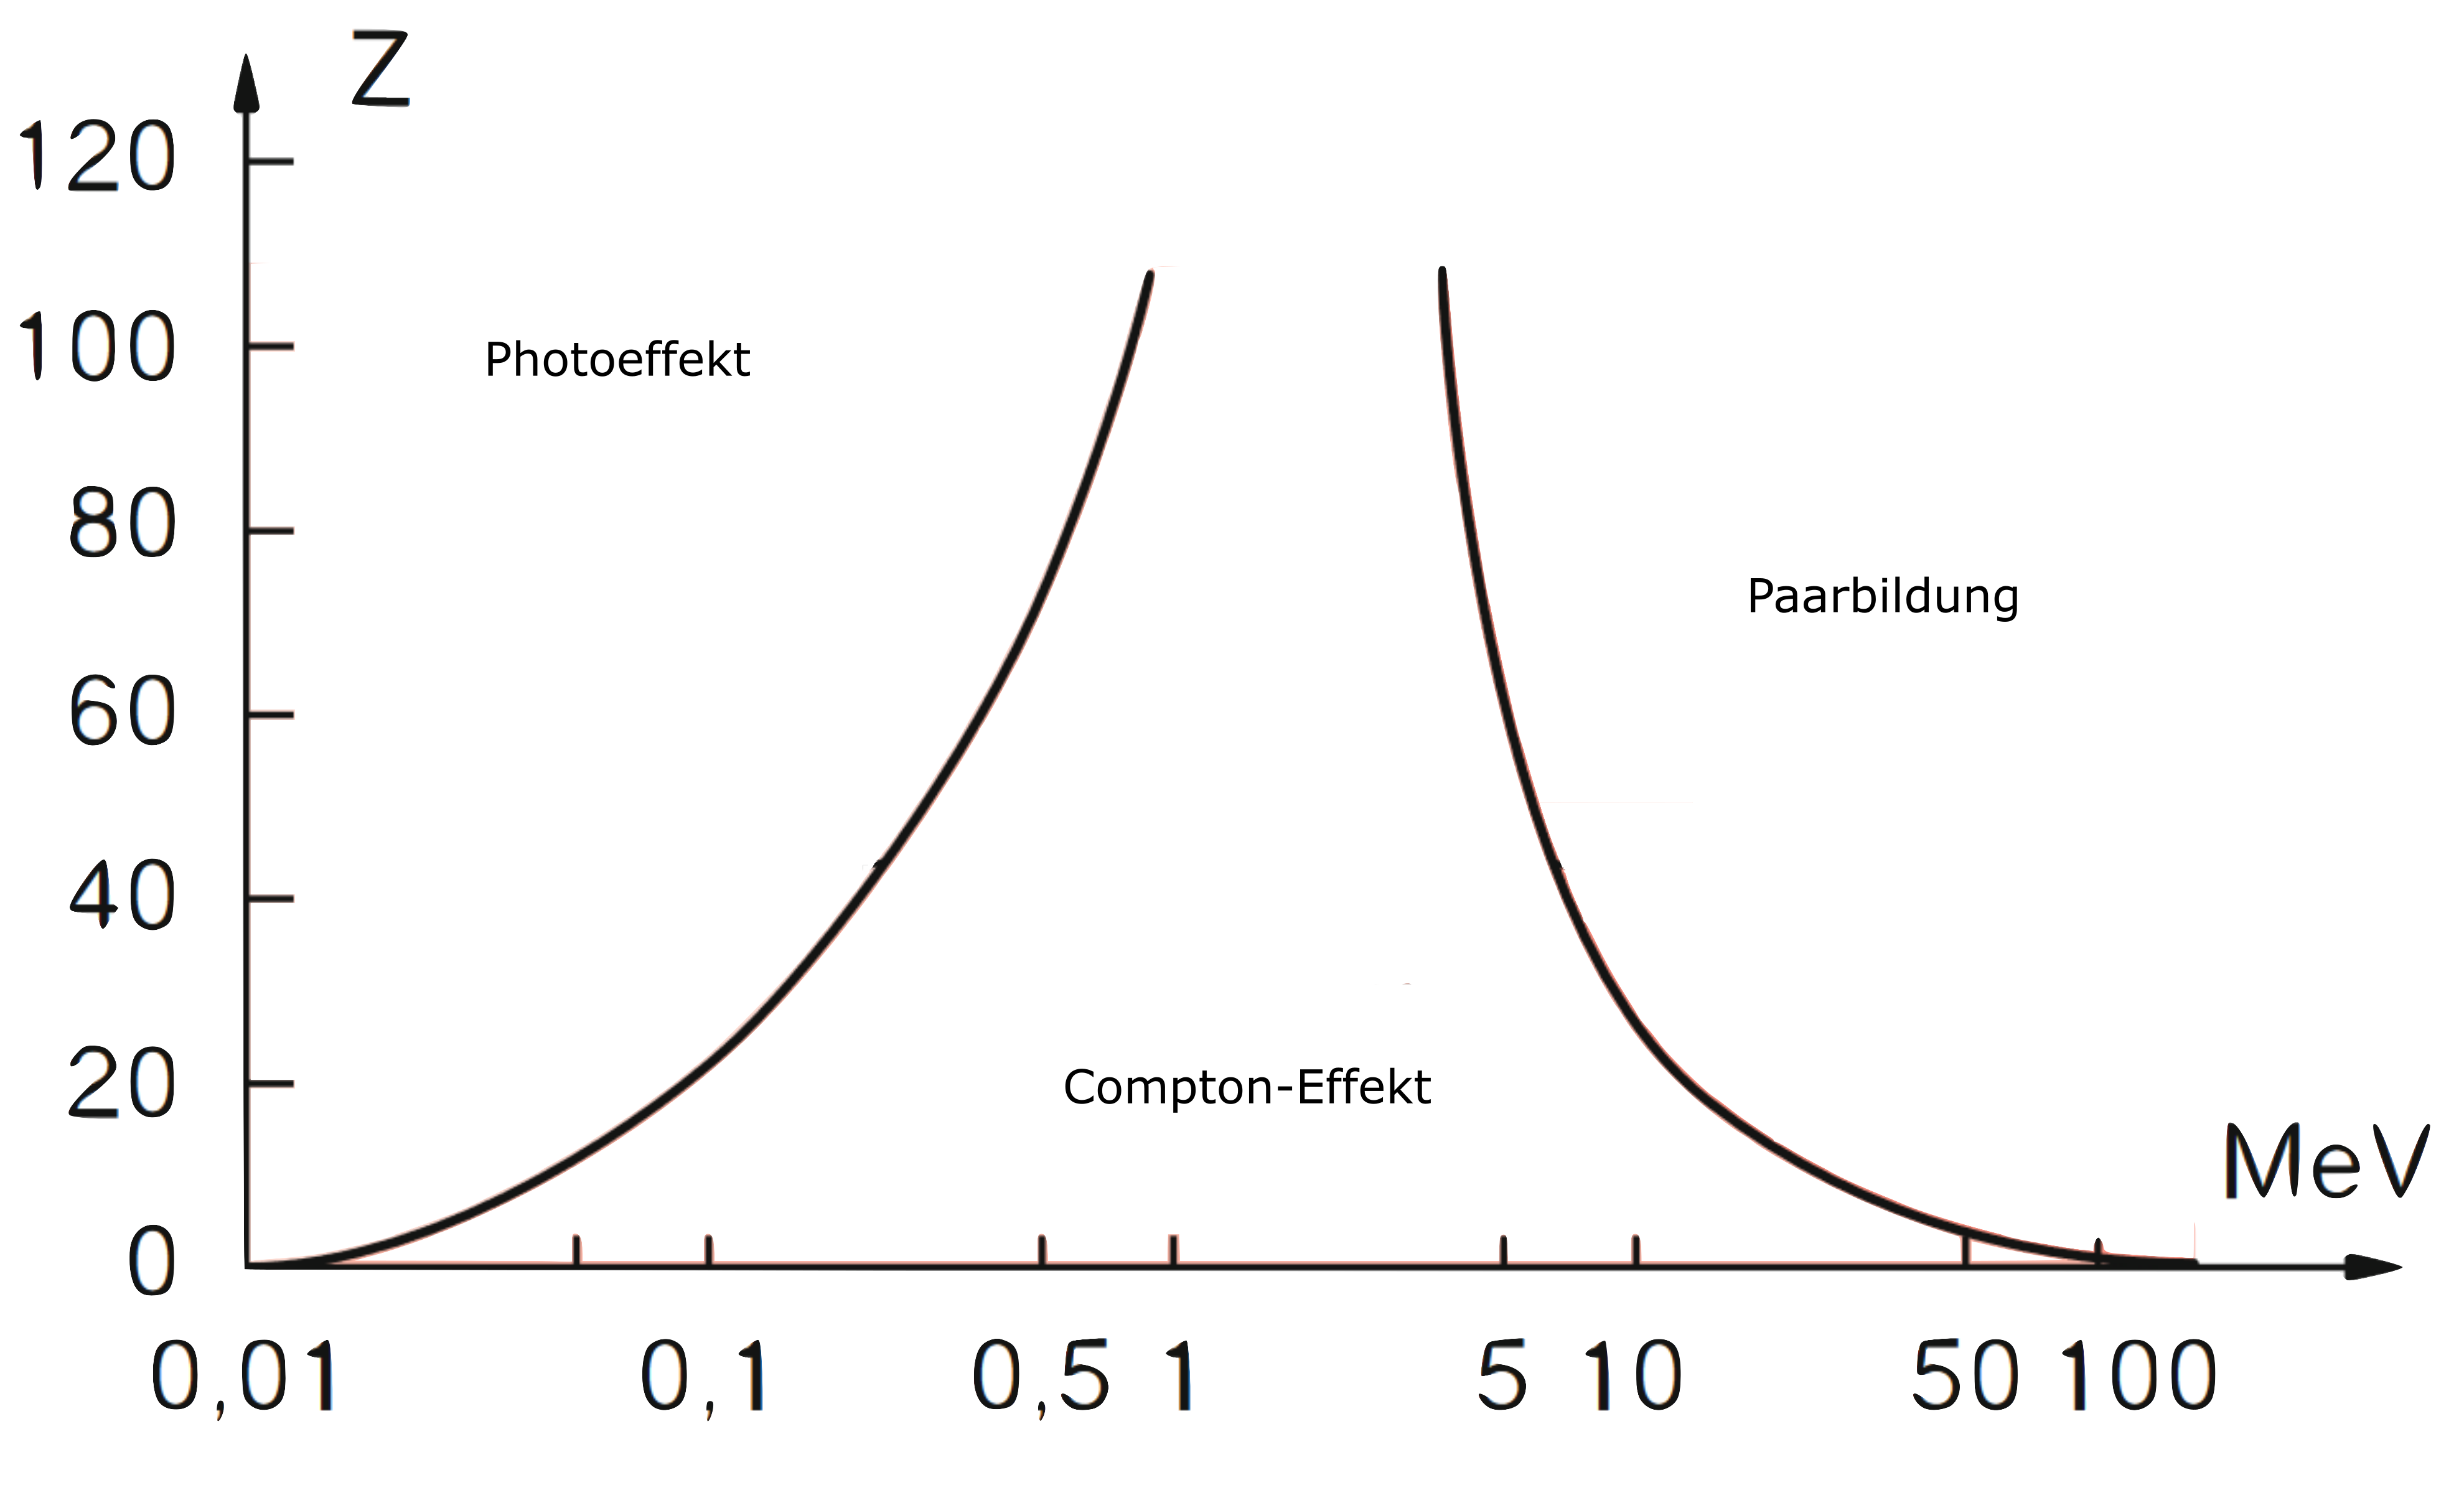
\includegraphics[scale=0.25]{PhotoQuerschnitte.png}
		\caption{Dominante Wechselwirkungen von Photonen in Abhängigkeit von der Kernladungszahl $Z$ des Absorbermaterials und der Photonenenergie. Die durchgezogenen Linien markieren die Grenzbereiche der dominierenden Effekte (modifiziert nach \cite{DemtroderKerne})}
		\label{fig:WirkungsquerschnittePhotonen}
	\end{figure}
	
		\subsubsection{Photoelektrischer Effekt}
		Der photoelektrische Effekt beschreibt die Absorption eines Photons durch ein gebundenes Elektron, wodurch das Atom angeregt oder ionisiert wird. Dieser Effekt dominiert im niederenergetischen Bereich (siehe Abbildung \ref{fig:WirkungsquerschnittePhotonen}). Mit der Bindungsenergie $\phi_{\text{A}}$ des Elektrons gilt für die Energie des auslösten Elektrons:
		\begin{equation*}
			E_{e^{-}}= E_{\gamma}-\phi_{\text{A}}
		\end{equation*} 
		
		\noindent Der Wirkungsquerschnitt ist sowohl kernladungszahl- als auch energieabhängig und tritt besonders stark bei Energien auf, die den Absorptionskanten der Atome entsprechen, insbesondere bei Atomen mit hoher Kernladungszahl  \cite{Leo}.
		
		
		\subsubsection{Compton-Streuung}
		Compton-Streuung ist die Streuung eines Photons an einem lose gebundenen Elektron. Ein Teil der Photonenenergie wird dabei auf das Elektron übertragen, das Photon wird nicht absorbiert. Man unterscheidet zwischen Rayleigh-, Thomson- und Compton-Streuung. Diese Phänomene werden durch die Klein-Nishina-Formel beschrieben, wobei die klassische Streuung den niederenergetischen Grenzfall der Compton-Streuung darstellt. Der Wirkungsquerschnitt der Compton-Streuung ist primär energieabhängig  \cite{Leo}:
		\begin{equation*}
			{\displaystyle \dv{\sigma}{\Omega}={\frac {1}{2}}{\frac {\alpha ^{2}}{m^{2}}}\left({\frac {E'}{E}}\right)^{2}\left({\frac {E'}{E}}+{\frac {E}{E'}}-\sin ^{2}\theta \right)}
		\end{equation*}
		wobei $\theta$ den Streuwinkel bezeichnet, $\alpha\approx 1/137$ die Feinstruktur-Konstante und $E^{\prime}$ die Energie des gestreuten Photons. Als ein Fall der elastischen Streuung existiert ein eindeutiger Zusammenhang zwischen der deponierten Energie und dem Streuwinkel.
		
		\subsubsection{Paarbildung}
		Photonen deren Energie einen Wert von $1,22\ \si{MeV}$ überschreiten, können sich im Feld eines Kerns zu Elektronen-Positronen-Paaren umwandeln. Eine Umwandlung ohne einen dritten Wechselwirkungspartner ist aufgrund der Impulserhaltung nicht möglich. Paarbildung wird damit nur für hochenergetische Strahlung relevant. Der Wirkungsquerschnitt skaliert mit \cite{DemtroderKerne}:
		\begin{equation*}
			\sigma \propto Z^{2}\ln(E_{\gamma})
		\end{equation*} 
		
		
	\newpage
	
	\subsection{Sekundärionisation}	\label{chap:Sekundär}
		Nach der Primärionisation durch das tatsächliche Detektionsereignis gibt es einige Effekte, die zu weiteren Ionisationen durch dasselbe Ereignis beitragen können. In diesem Zusammenhang spricht man von Sekundärionisationen. Ein Verständnis dieser Effekte ist fundamental für die korrekte Beurteilung der Arbeitsparameter von Detektoren (siehe Abschnitt \ref{sec: Parameter}).
		
		\subsubsection{Lokale Clusterbildung}
			Wird ein Elektron-Ionen-Paar durch Strahlung erzeugt, hat dieses Elektron oft noch so viel Energie, dass weitere Stoßwechselwirkungen mit den Atomen zu Sekundärionisationen führen können. Es bildet sich ein lokales Cluster aus Elektronen, die zu einem Detektionsereignis gehören, da der Ionisationsprozess so lange geht, bis die Energie des Elektrons für weitere Ionisationen nicht mehr ausreicht. Bei bekannter Ionisationsenergie des Mediums kann die Zahl der durch ein Detektionsereignis erzeugten Elektronen-Ionen-Paare kann wie folgt approximiert werden \cite{Sauli_Multiwire}:
			\begin{equation} \label{eq:Primärionisation}
				N_{\text{e}}=\frac{E_{\gamma}}{\phi_{\text{ion}}}
			\end{equation}	
			Der Wert, der aus dieser Formel folgt, ist offenbar ein Erwartungswert. Da die Wechselwirkungsprozesse statistischer Natur sind, fluktuiert die Zahl der erzeugten Elektronen-Ionen-Paare gemäß einer Polya-Verteilung \cite{ottnad}.
		
		\subsubsection{Penning-Effekt}
			Man kann nun ein anderes Molekül in das Medium geben, dessen Ionisationsenergie unterhalb der Anregungsniveaus des ursprünglichen Mediums liegt. Auf diese Weise kann man die Energie, die in Anregungen \enquote{verloren} geht wiederum durch Stoßwechselwirkungen zwischen den Atomen im Elektronen-Ionen-Paare umwandeln. In dieser Gasmischung wird die Effektive Ionisationsenergie quasi heruntergesetzt, sodass mehr Ionisationen stattfinden. Man bezeichnet dieses Gas als Quencher und den illustrierten Prozess als Penning Effekt \cite{ottnad}.
			
		\subsubsection{Auger-Meitner-Effekt}
			Im Kontext des Photoeffektes ist es wahrscheinlich, dass das ausgelöste Elektron aus einer unteren Schale stammt. Neben der Rekombination unter Emission von Strahlung oder internen Übergängen unter Photonenemission ist auch ein strahlungsloser interner Übergang möglich. Dabei kann ein weniger stark gebundenes Elektron der äußeren Schalen auf die innere zurückfallen und seine Energie an ein anderes Elektron im System abgeben, was zu einer weiteren Ionisation führen kann \cite{Sauli_Multiwire}. 
			
		\subsubsection{$\delta$-Elektronen und nicht-lokale Clusterbildung}
			Die statistische Natur der Wechselwirkungsprozesse erlauben es, dass ein ein hochenergetisches freies Elektron entstehen kann, das durch das Medium propagiert und in Übereinstimmung mit einer Modifizierten Bethe-Bloch-Formel \cite{Leo} Energie verliert. Hierbei können weitere Elektronen-Ionen-Paare erzeugt werden, die Position dieser Sekundärerzeugung muss allerdings nicht mit dem Ort der Primärionisation übereinstimmen, sondern kann deutlich entfernt stattfinden. Daher können mehrere Cluster entstehen, die zu einem Ereignis gehören. Delta-Elektronen können daher nicht nur die Ortsauflösung des Detektors beeinflussen, sondern auch für größere Fluktuationen bei der Messung der deponierten Energie sorgen.
			
		\newpage	
		
	\section{Bewegungen von Ladungen}		
	Wenn Elektronen-Ionen-Paare erzeugt wird, müssen diese gemessen werden, um daraus Erkenntnisse über die Strahlung zu gewinnen. Dafür müssen die Ladungen von der Rekombination aufgehalten und getrennt werden, weswegen die Bewegung von Ladungsträgern und damit verbundene Größen definiert und verstanden werden müssen.\\
	Die Bewegung eines Ladungsträgers setzt sich zusammen aus der Eigenbewegung des Teilchens, die durch zahlreiche Stöße in thermische Bewegung (Diffusion) übergeht und die Driftbewegung in elektromagnetischen Feldern.
	
		\subsection{Diffusion}	
		Ohne Elektrische Felder bewegt sich das Elektron entsprechend der Energie- und Impulserhaltung nach der Ionisationswechselwirkung. Durch die Stöße mit den Gasatomen wird die Bewegung verlangsamt und so umgelenkt, dass die Bewegung eines Elektronenensembles nunmehr ungerichtet ist, die Elektronenwolke diffundiert. Die Beschreibung dieser Prozesse im Rahmen der kinetischen Gastheorie zeigt, dass die räumliche Verteilung um den Primären Ionisationspunkt gauß'sch ist, wobei die räumliche Ausdehnung aus der Standardabweichung der resultierenden Verteilung abgeschätzt werden kann \cite{Sauli_Multiwire}. Die Diffusionsbewegung begrenzt also die räumliche Auflösung des Detektors auf natürliche Weise.\\
		\\
		Die Bewegung des Teilchens lässt sich durch die mittlere freie Weglänge beschreiben, die als Maß für die Strecke fungiert, die ein Teilchen zwischen zwei Wechselwirkungen zurücklegt. Sie ergibt sich aus der Teilchendichte des Mediums $n$ und dem Wirkungsquerschnitt $\sigma$ über:
		\begin{equation}
			\lambda=\frac{1}{n\sigma}
		\end{equation} 
		Insbesondere lässt sich die mittlere freie Weglänge als Maß für die Interaktionsrate für Ionisation und Rekombination verwenden \cite{Sauli_Multiwire}. Für Elektronen ist die thermische Geschwindigkeit und die Mittlere Freie Weglänge mehrere Größenordnungen größer als für Ionen, es ist daher deutlich angemessener die Elektronen für die Signalerzeugung am Detektor zu Verwenden.
		
		\subsection{Bewegung von Ladungsträgern in Feldern}\label{sec:Bewegung in Feldern}
		Auf bewegte Ladungen in elektromagnetischen Feldern wirkt die Lorentzkraft und beschleunigt das Elektron entlang oder senkrecht zur Bewegungsrichtung. In der folgenden Detektorkonfiguration (siehe Abschnitt [GEM Design]) wird kein magnetisches Feld verwendet. Daher wird im Folgenden der Spezialfall mit Lorentzkraft für $\vec{B}=0$ betrachtet. Die Bewegung setzt sich zusammen aus den Stößen mit den Gasatomen und dem Drift im elektrischen Feld, das Problem wird damit beschrieben durch einen Spezialfall der Langevin-Gleichung \cite{Schwabl}:
		\begin{equation*}
			m \dot{v}= q \vec{E}- f(t)
		\end{equation*}
		Wobei $m$ die Teilchenmasse, $q$ die Ladung und $\vec{E}$ das elektrische Feld beschreibt, während $v$ die Geschwindigkeit und $f(t)$ eine zeitabhängige Kraft ist, die aus den Stoßwechselwirkungen resultiert. Nach einer charakteristischen Zeit $\tau$ stellt sich indes ein Gleichgewicht ein, mit dem die Bewegung näherungsweise gleichförmig wird, für diesen Fall löst sich die Langevin-Gleichung dann über:
		\begin{equation*}
			\vec{v}= \mu \vec{E}
		\end{equation*}
		Wobei man $\mu=q/m \tau$ als Beweglichkeit des Teilchens bezeichnet, die mit der mittleren Stoßzeit $\tau$ und so mit der mittleren freien Weglänge zusammenhängt \cite{ottnad}. In erster Näherung wird damit klar, dass die Geschwindigkeit und so die kinetische Energie ausschließlich vom anliegenden Elektrischen Feld abhängt.
		
		\newpage
	\section{Gasdetektorklassen}
		Mit dem Wissen über die Erzeugung und das Verhalten von freien Ladungsträgern in Gasen ist es nun möglich die Grundzüge der Gas-Detektorklassen zu erörtern. Hierbei werden zunächst allgemeine Anmerkungen über die grundlegenden Konzepte gemacht, wobei im Besonderen auf den Anwendungsbereich und Limitationen geachtet wird, formale Überlegungen zum Aufbau werden indes nicht gemacht, da der Konzeptionelle Aufbau im Allgemeinen recht ähnlich ist, sofern es keine besonderen Detektorkonzepte benötigt. Die Hauptunterscheidung der Klassen liegt in der Betriebsspannung \cite{Leo}.
		
		\subsection{Ladungsmultiplikationsmechanismen} \label{sec:Ladungsmultiplikation}
			Wenn die kinetische Energie eines Teilchens die Ionisationsenergie eines Atoms überschreitet, können Ionisaationen auftreten. Ausgehend davon, dass die kinetische Energie geladener Teilchen in Feldern wesentlich von den anliegenden Feldern abhängt (siehe Abschnitt \ref{sec:Bewegung in Feldern}), kann das Feld so eingestellt werden, dass Sekundärionisationen stattfinden. Je nach Feldstärke und Größe der Multiplikationsregion können dann auch in derselben Region ausgelöste Elektronen bereits zur Verstärkung der Elektronenwolke beitragen, es entsteht eine Elektronenlawine \cite{Townsend}, \cite{Leo}.\\
			\\
			Die Zahl der Ladungsträger, die pro Längeneinheit entstehen sind eng mit der Zahl der Wechselwirkungen und damit mit der mittleren freien Weglänge verbunden. Man bezeichnet die Zahl der entstehenden Ladungsträger als ersten Townsend-Koeffizienten, für den gilt:
			\begin{equation*}
				\alpha=\frac{1}{\lambda}
			\end{equation*}
			Die Wachstum der Elektronenlawine ist offenbar ein exponentieller Prozess, wobei der Townsend-Koeffizient sowie die Länge der Lawinenentstehungsgebietes relevante Größen sind, um die Lawinenentstehung zu beschreiben. Als Multiplikationsparameter wird die Verstärkung (im Folgenden Gain) definiert, die die Zahl der entstehenden Ladungen beschreibt:
			\begin{equation}
				G=\frac{N}{N_{0}} = e^{\alpha d}
			\end{equation}
			Der erste Townsendkoeffizient ist abhängig vom verwendeten Medium und steigt mit der Feldstärke an, das Verhalten des Koeffizienten als Funktion der Feldstärke ist in Abbildung  \textcolor{blue}{Abbildung: Townsend-Koeffizienten} zu sehen. Um Gasentladungen zu verhindern, kann die Zahl der Elektronen im Verstärkungsvolumen nicht beliebig ansteigen. Ein empirisch bestimmtes Limit für einen stabilen Betrieb ist das Raether-Limit nach dem gilt $\alpha d<20$ \cite{Sauli_Multiwire}.
			
			
			\newpage
		\subsection{Ionisations- und Proportionalkammern} \label{sec:IonisationsundProportionalkammern}
			Grundsätzlich unterscheidet man für Gasdetektoren, die nicht nur zum Nachweis, sondern auch zur Vermessung der Strahlung genutzt werden können, Ionisations- und Proportionalkammern.\\
			 Ionisationskammern werden von elektrischen Feldern durchzogen, die nicht stark genug sind, um systematisch Ladungsmultiplikation auszulösen und dennoch (fast) alle entstehenden Elektronen-Ionen-Paare trennen und zur Ausleseelektronik zu überführen. Wird die Auslese segmentiert, ist es prinzipiell möglich die Spur des Teilchens zu rekonstruieren, in der Praxis sind die Signale allerdings zu schwach um adäquat vermessen zu werden. Es braucht eine zusätzliche Verstärkung, bevor die Elektronen die Auslese erreichen. Ausgehend davon, dass die Funktionsweise der Spurrekonstruktion für diese Arbeit nur peripher relevant ist, wird auf eine extensive Diskussion verzichtet, stattdessen reicht ein Verweis auf die dafür vorgesehene Fachliteratur \textcolor{red}{Zitation: Funktionsweise TPC}\\
			\\
			 Um die Unzulänglichkeiten der Ionisationskammer zu kompensieren, kann man das Elektrische Feld so wählen, dass eine Ladungsmultiplikation einsetzt, eine Minimalsbschätzung kann hierbei durch die Townsend-Koeffizienten geschehen, nach Abbildung \textcolor{blue}{Abbildung: Townsend-Koeffizienten} beginnt das Multiplikationsregime bei [ZAHLENWERT].\\
			 \\
			  Bei alleiniger Nutzung einer Proportionalkammer ist die Verstärkung im Allgemeinen auch Funktion des Entstehungsortes des Elektronen-Ionen-Paares. Um diese Limitation zu überwinden, können die Ionisationszone und die Verstärkungszone durch eine vorgelagerte Ionisationskammer getrennt werden, wodurch die Abhängigkeit vom Entstehungsort wegfällt, da alle Elektronen an der gleichen Stelle an die Verstärkungsregion übergeben werden.\\
			  \\
			  Eine weitere Limitation tritt genau dann zu Tage, wenn die Felder zu groß gewählt werden. In diesem Fall ist die Verstärkung so stark, dass eine wohllokalisierte Ladungszone aus Ionen entsteht, die das elektrische Feld verzerrt und so weitere Multiplikation temporär unterbinden kann, da sie deutlich langsamer als Elektronen driften. In diesem Fall encoded das Ausgangssignal keine genaue Information zu der im Detektor deponierten Energie, die Proportionalität des Detektors geht verloren, sodass es eine natürliche Gain-Limitation gibt, mit der der Betrieb als Proportionalkammer möglich ist.
			 
			 \newpage
		\subsection{Parameter von Gasdetektoren} \label{sec: Parameter}
			Zum Abschluss des Grundlagenkapitels für Gasdetektoren sollen nun einige finale Überlegungen zu generellen Eigenschaften und Parametern von Gasdetektoren angestellt werden. Im folgenden werden demnach die Ionisationseigenschaften des Aktiven Mediums, sowie die Energieauflösung von Gasdetektoren diskutiert,
			
			\subsubsection{Wahl des Gases}
				Die Townsend-Koeffizienten sind aufgrund der unterschiedlichen Ionisationsnergien der verschiedenen Elemente materialspezifisch \textcolor{blue}{Abbildung: Townsend-Koeffizienten}. Die Ladungsverstärkung ist demnach abhängig von der Wahl des Aktiven Mediums und ist ihrerseits Thema kontinuierlicher Untersuchung \cite{GAS_MIX}. 
				Diese Untersuchungen erlauben nun eine informierte Wahl des Aktiven Mediums, indem man einige Auswahlkriterien definiert und die Mixtur auswählt, die diese Kriterien erfüllt:\\
				\\
				Ausgehend davon, dass das aktive Medium immer einer externen Energie ausgesetzt ist, sind chemische Reaktionen mit der Detektorbegrenzung oder dem Quencher-Gas im Allgemeinen nicht auszuschließen. Entsprechend können sich durch Reaktionen Alterungserscheinungen ausbilden, die den Detektorbetrieb beeintächtigen \cite{Ageing}. Daher ist ein möglichst reaktionsträges Element als Basis des aktiven Mediums zu verwenden. Edelgase sind in dieser Hinsicht bestens geeignet.\\
				Unter den Edelgasen gibt es neben Kriterien wie Verfügbarkeit und damit verbunden den Kosten noch andere physikalische Einschränkungen, die die Kandidaten für die Basis des aktiven Mediums begrenzen. Neben einer hinreichend kleinen Ionisationsenergie sind daher Diffusionskoeffizienten und Molekülmobilität weitere Einschränkungen an das Gas. \\
				Um eine möglichst große Elektronenausbeute zu garantieren, wird im folgenden Argon verwendet, das Argon vergleichsweise niedrige Ionisationsenergien hat (siehe Tabelle \ref{tab:Ionisationsenergien}), wobei CO$_{2}$ als Quench-Gas beigemischt wird. Das Mischungsverhältnis der Gase wird im Folgenden $90\%-10\%$ sein, dies erlaubt eine adäquate Ausnutzung der in \ref{chap:Sekundär} erwähnten Effekte.
				
				\begin{table}[h]
					\centering
					\begin{tabular}{|c|c|c|c|c|c|c|c|c|}
						\hline
						Gas & He & Ne & Ar & Kr & Xe & \ce{CO_{2}} & \ce{CH_{4}} & $\ce{Ar-CO_{2}} (90-10)$\\
						\hline
						$W_{\text{ion}} / \si{eV}$ & 42,7 & 36,8 & 26,4 & 24,1 & 21,9 & 34,5 & 29,2 & 27,2\\
						\hline
					\end{tabular}
					\caption{mittlere Ionisierungsenergie für ausgewählte Gase nach \cite{Gas_Energien} }
					\label{tab:Ionisationsenergien}
				\end{table}
				
				\newpage
			\subsubsection{Energieauflösung eines Detektors}
				Wird monochromatische Strahlung in einen Detektor gestrahlt, sollte dieser ein Signal erzeugen. welches zu der Energie des monochromatischen Strahlung passt. Das Messergebnis ist allerdings keinesfalls eine diskrete Linie, sondern hat ein Semi-Gaußprofil. Für einen Gasdetektor (ohne Ausleseelektronik) gibt es einige Mechanismen, die zu dieser Form beitragen. Die wichtigsten sollen hier kurz umrissen werden:
				\begin{enumerate}
					\item \textbf{Primär-Ionisationsfluktuationen}: Die Zahl der durch ein Photon der Energie $E_{\gamma}$ erzeugten Elektronen-Ionen-Paare kann mit Gleichung \ref{eq:Primärionisation} abgeschätzt werden. Aus der statistischen Natur der Prozesse folgen allerdings Fluktuationen um den Mittelwert. Um diese adäquat abzuschätzen, muss beachtet werden, dass die Ionisationsprozesse in diesem Fall nicht gänzlich unabhängig sind, sodass die Abschätzung der rein statistischen Fluktuationen (Poisson) um den Fano-Faktor $F$ korrigiert werden muss \cite{ottnad},\cite{Leo}. Insgesamt ergibt sich dann eine Energieauflösung der folgenden Form: 
					\begin{equation*}
						R=\frac{\sqrt{F}}{N}
					\end{equation*}
					\item \textbf{Verstärkungsfluktuationen}: In Proportionalkammern kommt eine Fluktuation für die Sekundärionisationsprozesse der einzelnen Elektronen dazu. Unter der Annahme, dass das $i$-te Elektron eine Zahl $G_{i}$ von Sekundärelektronen produziert, stellt sich die Gain offenbar als Mittelwert der Sekundärelektronen über alle Prozesse dar. Die Fluktuationen aus dem einzelnen Prozess pflanzen sich dann entsprechend auf die Gain fort. Unter der Annahme, dass die Fluktuationen $\sigma_{\text{G}_{i}}$ gleich sind gilt demnach:
					\begin{equation*}
						\sigma_{\text{G}}= \frac{\sigma_{\text{G}_{i}}}{\sqrt{N}}
					\end{equation*}
				Für den Anteil durch die Verstärkungsflukturationen gilt demnach dann \cite{ottnad}:
				\begin{equation*}
					R=\frac{\sigma_{\text{G}}}{G}
				\end{equation*}
				\end{enumerate}
			Die Kombination beider Fluktuationsbeiträge ergibt zusammen mit einem Rauschbeitrag durch elektronisches Rauschen die Energieauflösung. Experimentell bestimmt sie sich durch die Auswertung eines wohlbekannten Spektrums, bei dem man eine bekannte Linie messen kann, um anschließend eine Kurve daran anzupassen und aus der Halbwertsbreite folgende Abschätzung zu verwenden:
				\begin{equation*}
					R=\frac{\Delta E}{E}= \frac{\sigma_{{\text{Photo}}}}{\mu_{\text{Photo}}}
				\end{equation*}
			Detaillierte Darstellungen zur Verwendeten Strahlung, mit der diese Bestimmung durchgeführt werden finden sich in Abschnitt  \ref{sec:Fe55}. In diesem Zusammenhang wird die Nomenklatur der einzelnen Signalanteile sowie die Benennung der hier bereits verwendeten Formelzeichen durchgeführt.
			
			

\chapter{Gas Electron Multiplier}
Ordinäre Proportionalkammern sind natürlichen Problemen und Limitationen unterworfen, die in Abschnitt \ref{sec:IonisationsundProportionalkammern} allgemein diskutiert wurden. Für präzisere Untersuchungen sind jedoch elaboriertere Detektorkonzepte erforderlich, die beispielsweise Orts- und Spurrekonstruktion ermöglichen, um so Zerfallsprozesse zu berücksichtigen. Eine frühe Möglichkeit dies zu realisieren waren Vieldraht-Proportionalkammern (MWPC), bei denen die Rekonstruktion durch die Verwendung und Auslese von vielen Proportionalzählern ermöglicht wurde. Eine extensive Erklärung der Funktionsweise findet sich in \cite{Sauli_Multiwire}.\\
Um eine präzisere Rekonstruktion zu gewährleisten, ist es sinnvoll, die Auslesestruktur weiter zu segmentieren. Präzisere Ergebnisse sind insbesondere dann möglich, wenn auch die Verstärkerstufen mikrostrukturiert sind. In diesem Kontext treten die Gas Electron Multiplier (GEMs) auf, die dies ermöglichen. Im folgenden Kapitel soll das Konzept dieser Detektorgeometrie diskutiert werden, um auf diese Weise die weitreichenden Vorteile dieser Anordnung zu erläutern.

\section{Aufbau und Funktionsweise einer GEM-Verstärkungsstufe} 
  GEMs sind zunächst einmal mikrostruktuierte Versionen von Proportionalkammern. Wegen ihrer Bauweise können sie hintereinander geschaltet werden, sodass wir im folgenden von Verstärkerstufen sprechen. GEM-Verstärkerstufen sind dünne Polyamidfolien, die beidseitig mit Kupfer beschichtet sind. Die Strukturierung der Stufe erfolgt dadurch, dass Löcher in die Folien geätzt werden, sodass sich eine hexagonale Struktur ausbildet (siehe Abbildung \ref{fig:Draufsicht}). Der Abstand zweier paarweise benachbarter Löcher, im Folgenden Pitch, ist daher stets gleich.\\
   Die Eigenschaften der Foliengeometrie, insbesondere Pitch und Lochradien, wurden in der Vergangenheit umfassend untersucht \cite{Sauli_Übersicht}. Basierend auf diesen Untersuchungen haben sich spezifische Konfigurationen etabliert, und entsprechend dieser Konvention werden GEM-Folien im Standardformat verwendet, die Parameter der Folie sind als Querschnitt der Folie in Abbildung \ref{fig:Querschnitt} zu sehen.

	\begin{figure}[h]
		\centering
		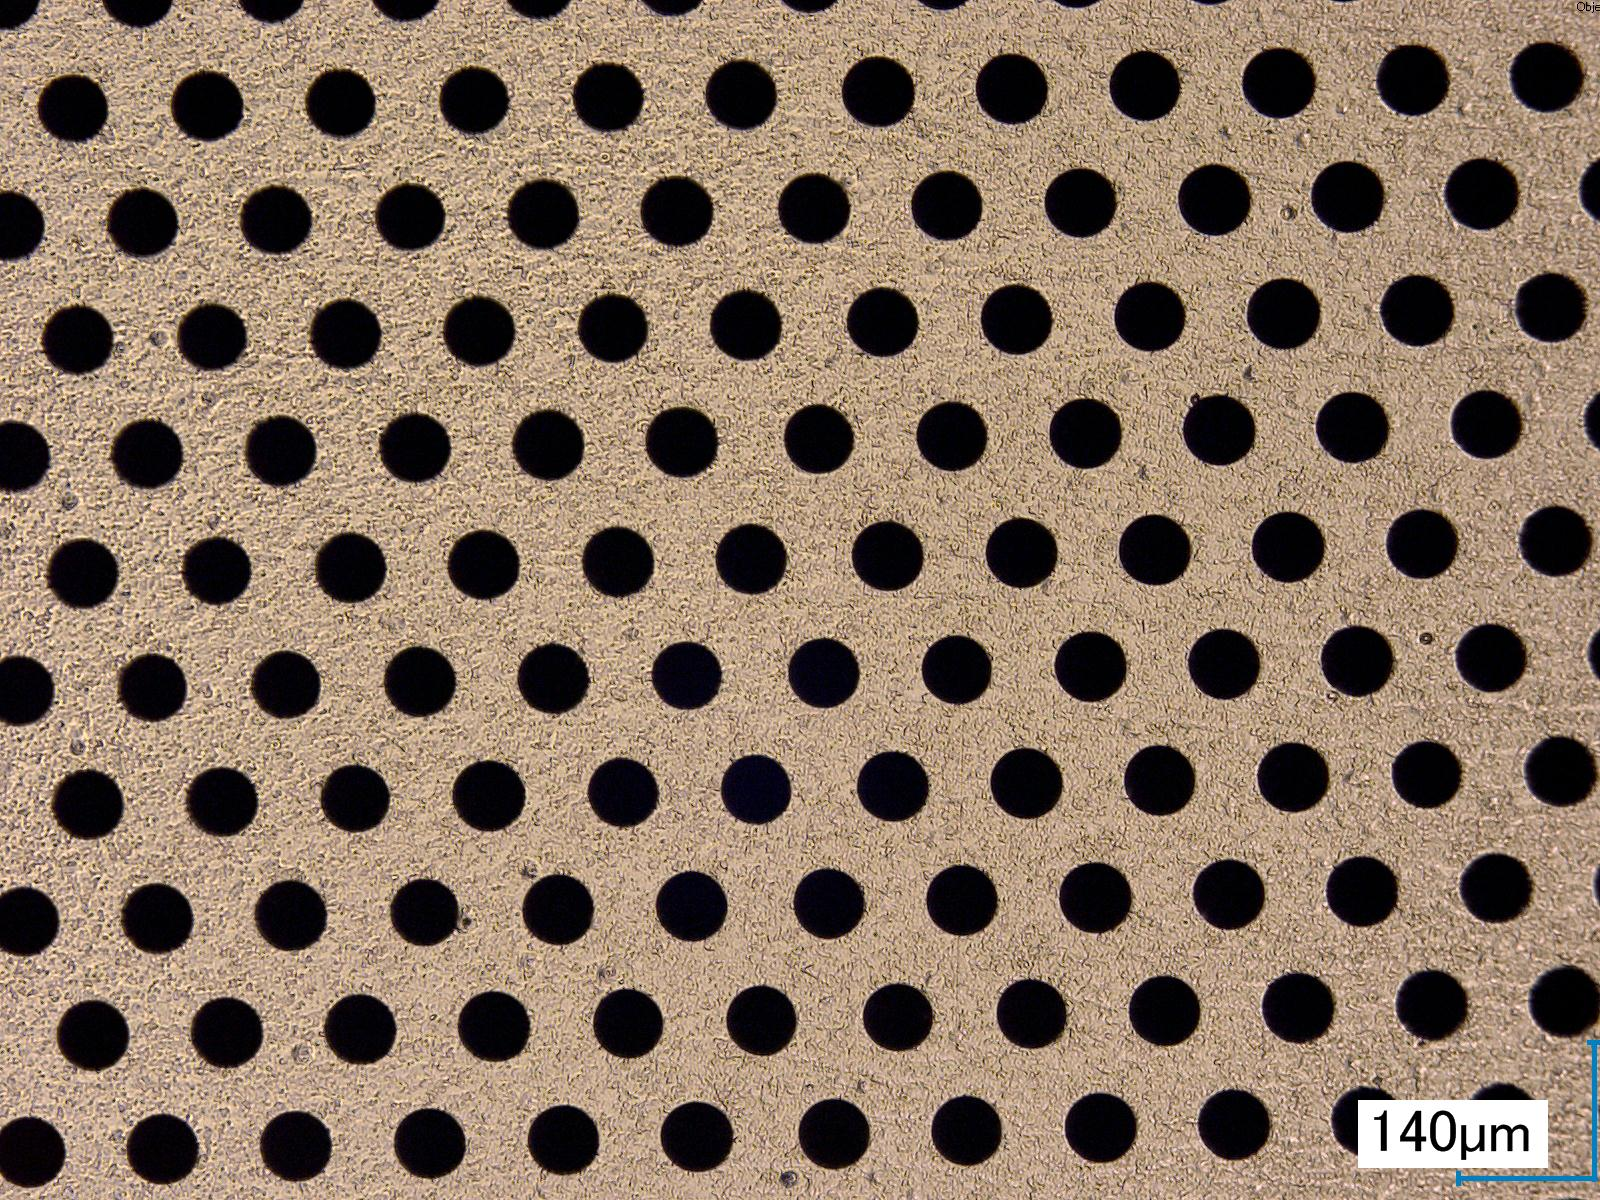
\includegraphics[scale=0.15]{Topside_UpperLeft.jpg}
		\caption{Draufsicht auf Folienausschnitt aufgenommen mit einem Digitalmikroskop Modell VHX-200 \cite{MikroskopReinraum}, ausgezeichnet ist der ein Maßstab von $140 \si{\mu m}$}
		\label{fig:Draufsicht}
	\end{figure}

	\begin{figure}[h]
		\centering
		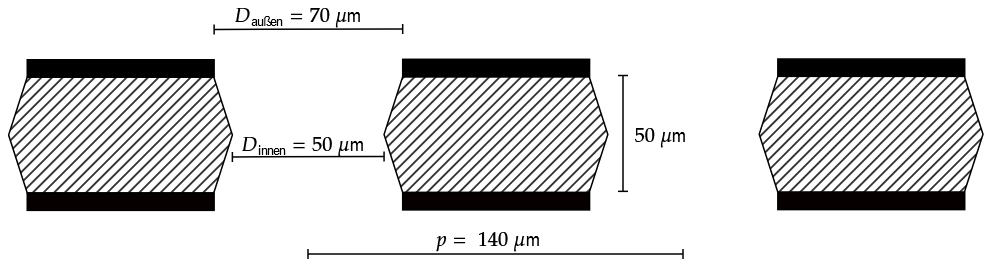
\includegraphics[scale=0.5]{Querschnitt GEM.png}
		\caption{Querschnitt der Folie}
		\label{fig:Querschnitt}
	\end{figure}
		
		
		
\noindent Die wesentliche Stärke dieses Ansatzes liegt darin, dass eine vergleichsweise kleine Spannung zwischen den Kupferplatten zu großen Feldern in den Löchern führt. So führt bspw. eine Potentialdifferenz von $100\ \si{V} $ zu einem Feld der Größenordnung von $20.000\ \si{V/cm}$. Ein Vergleich mit dem Townsend-Koeffizienten (siehe Abbildung \textcolor{blue}{Townsend-Koeffizient}) zeigt, dass in diesem Bereich eine starke Ladungsmultiplikation auftritt. Durch die starke räumliche Begrenzung der einzelnen Verstärkungvolumina wird der störende Einfluss der Ionen reduziert, da die Distanzen, die die Ionen zurücklegen müssen, um an einer Elektrode mit einem Elektron zu rekombinieren vergleichsweise gering ist. Auf diese Weise verläuft die Multiplikation homogen. Um das Einzusehen, sind die Äquipotentialflächen eines GEM-Feldes in Abbildung \textcolor{blue}{GEM-Feld} dargestellt. Diese Konstruktion erlaubt es demnach bei potentiell höheren Verstärkungen zu operieren, ohne dass Informationen über die im Detektor deponierte Energie verloren gehen. \\
\\
Da es sich bei den einzelnen GEM-Löchern im Wesentlichen um Proportionalkammern handelt, gelten die in Abschnitt \ref{sec:IonisationsundProportionalkammern} diskutierten Grenzen für jedes der Löcher individuell. Es ist allerdings so, dass die Verstärkung in den Folien, also entsprechend elektronisch getrennt von der Ausleseelektronik insofern vorteilhaft ist, dass Gasentladungen die Ausleseelektronik im Allgemeinen nicht erreichen und sie so nicht zerstören können. Es ist allerdings möglich. dass Gasentladungen in den Löchern der Folie auftritt und auf diese Weise die Folie schädigt. Es ist also geboten die Folie bei moderater Verstärkung. in Einklang mit den diskutierten Limits zu verwenden.
			



\section{Multi-GEM-Strukturen}
	Neben den bisher erörterten Vorteilen wird das volle Potenzial von GEM-Stufen erst dann ausgeschöpft, wenn mehrere Stufen hintereinander geschaltet werden. Auf diese Weise können die Elektronen, die aus einer ersten Verstärkungsstufe hervorgehen, an eine zweite Stufe übergeben werden, um dort weitere Multiplikationsschritte zu durchlaufen. Dies ermöglicht das Erreichen hoher Verstärkungen mit geringerem Aufwand und reduziert somit die Häufigkeit von Gasentladungen. \\
	Die Übergabe zwischen den Verstärkungstufen erfolgt über Driftkammern. So werden Gasentladungen zwischen den Folien verhindert, und Diffusionseffekte sorgen dafür, dass die Elektronen aus einer Verstärkungsstufe nicht nur in ein einzelnes GEM-Loch der nachfolgenden Stufe gelangen, sondern in mehrere. Dies erlaubt es, das Raether-Limit für Proportionalkammern effektiv zu umgehen und höhere Verstärkungen zu erzielen, ohne das Risiko von Gasentladungen signifikant zu erhöhen. Eine solche Konfiguration wird als Multi-GEM-Detektor bezeichnet.\\
	\\
	 In Abbildung \ref{fig:Konzeptskizze GEM Aufbau} wird der schematische Aufbau eines Triple-GEM Detektors gezeigt. Hierbei ahmt die Abbildung die tatsächliche Struktur des verwendeten Setups nach, statt auf die konzeptionelle Funktionsweise zu setzen. Diese Anordnung der Folien ist Resultat zahlreicher Optimierungsversuche. In diesem Kontext hat sich gezeigt, dass der Störeinfluss durch die Ionen noch effektiver reduziert werden kann, wenn die Folien um $90^{\circ}$ gegeneinander rotiert werden. Dies limitiert die Ionen auf den Bereich zwischen zwei GEM-Folien und verhindert so erhebliche Störungen durch die Propoagation der Ionen durch den Detektor.
	
	\begin{figure}[h]
		\centering
		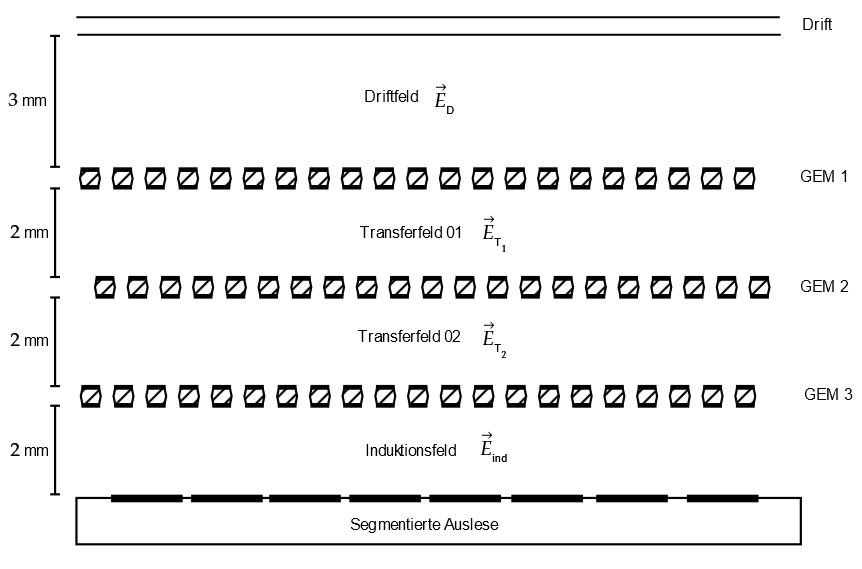
\includegraphics[scale=0.5]{Querschnitt Detektor.png}
		\caption{Querschnitt eines Triple-GEM Detektors mit segmentierter Ausleseelektronik. Die Abstände der einzelnen Stufen zueinander sind auf das verwendete Setup angepasst, zusätzlich wurde die Nomenklatur der Felder angepasst (modifiziert nach \cite{Sauli_Übersicht})}
		\label{fig:Konzeptskizze GEM Aufbau}
	\end{figure}
	
	
	\newpage

\section{Effektive Gain und Transfereffizienzen}
In einem Idealen System würden alle Elektronen, die bei der Verstärkung erzeugt werden auch in die nächste Verstärkerstufe und so zur Ausleseelektronik gelangen. In der Praxis ergeben sich im Wesentlichen drei Wege, über die Elektronen für die anderen Stufen verloren gehen können:
\begin{enumerate}
	\item Wechselwirkung mit der oberen Kupferplatte: Die Elektronen werden von dem GEM-Feld im Allgemeinen in das Loch gesaugt, es gibt jedoch einen Teil der Elektronen, die nicht eingesaugt werden, sondern von der Kupferplatte abgefangen werden. Diese Elektronen stehen offenbar nicht mehr für die Verstärkung zur Verfügung
	\item Verluste durch Polyamid-Interaktion: Elektronen, die in die Verstärkerstufe aufgenommen wurden, können von der Berandung der Löcher aufgenommen werden und stehen so nicht mehr zur Verfügung
	\item Wechselwirkungen mit der unteren Kupferplatte: Die Elektronen, die aus der Verstärkerstufe extrahiert werden, können bei der Extrahktion durch das GEM-Feld auf die untere Platte beschleunigt werden. Diese können dann offenbar nicht mehr weiterverwendet werden. 
\end{enumerate}
Physikalisch steht dahinter die Intuition, ob die Felder in einer Art zusammenwirken, die die Übergabe der Elektronen der Drift- und Transferfelder an GEM-Stufen begünstigen oder erschweren. Zu diesem Zweck definieren wir die Transfereffizienzen:
\begin{equation*}
	\epsilon_{\text{coll}}=\frac{N_{\text{gesammelt}}}{N_{\text{ein}}} \quad \epsilon_{\text{extr}}=\frac{N_{\text{extr}}}{N_{\text{extr}}+N_{\text{verl}}}
\end{equation*}
Hierbei bezeichnet die Kollekttionseffizienz $\epsilon_{\text{coll}}$ die Zahl der aus einer Stufe eingesammelten Ladungen normiert auf die Zahl der gesamt-einfallenden Ladungen und die Extraktionseffizienz $\epsilon_{\text{extr}}$ das Verhältnis der extrahierten Ladung normiert auf die Gesamtladung, die sich aus der extrahierten und der verlorenen Ladung zusammensetzt. Die Transfereffizienten verändern dabei offenbar die Verstärkung. Unter der Annahme, dass eine GEM-Stufe eine Absolute Verstärkung $G_{\textbf{abs}}$ hat, ergibt sich unter Verwendung der Transfereffizienzen folgender Zusammenhang:
\begin{equation}
	G_{\text{eff}}= \epsilon_{\textbf{coll}} \epsilon_{\text{extr}} G_{\text{abs}}
\end{equation}
Die effektive Verstärkung ist hierbei offenbar die Messbare Quantität und ist im Allgemeinen kleiner als die Absolute Verstärkung. Die Transfereffizienzen waren in der Vergangenheit bereits Thema von unterschiedlichen Verständnis und Optimierungsprozessen. In diesem Zusammenhang konnte gezeigt werden, dass die Transfereffizienzen vom Verhältnis der angrenzenden Felder abhängig ist. Insbesondere sind die Kollektionseffizienzen also abhängig von dem GEM-Feld und dem Feld, dass die Teilchen übergibt; die Extraktionskoeffizienten sind abhängig vom den GEM-Feldern und dem Feld, dass die Elektronen extrahiert.